%#########################1########################

 \cajita{%
Lactancia en niños menores de 5 años }%
{%
 }%
{%
 Niños menores de cinco años que lactaron alguna vez} %
{%
 República de Guatemala, 2008/2009, en porcentaje} %
{%
<<<<<<< HEAD
\small
%\ra{1.2}$\ $\\
\begin{tabular}{p{3.5cm}c}\hline
	\rowcolor{color2!0!white}&\\[-4mm]
	{\Bold   Característica}  & \textbf{Alguna vez recibió lactancia}\\
	\hline
	\rowcolor{color1!40!white} &\\[-4mm]
\rowcolor{color1!40!white}\textbf{Área geográfica}	&		\\
\rowcolor{color1!10!white}Urbana	&	94.4	\\
Rural	&	97.1	\\
\rowcolor{color1!40!white}\textbf{Región}	&		\\
\rowcolor{color1!0!white}Metropolitana	&	94.2	\\
Norte	&	95.9	\\
Nororiente	&	95.4	\\
Suroriente	&	93.7	\\
Central	&	96.5	\\
Suroccidente	&	97.1	\\
Noroccidente	&	97.3	\\
Petén	&	97.6	\\
\rowcolor{color1!40!white}\textbf{Categoría étnica de la madre}	&		\\
\rowcolor{color1!10!white}Indígena	&	97.1	\\
Ladino	&	95.2	\\
	\hline
	
\rowcolor{color1!0!white}	&\\[0.05cm]
\end{tabular}
}%
=======
}%
>>>>>>> origin/master
{%
 ENSMI 2008/2009} %


%#########################2########################

\cajita{%
	Duración de la lactancia según área de residencia}%
{%
}%
{%
	Duración de cualquier tipo de lactancia en niños menores de 2 años según área de residencia de la madre} %
{%
	República de Guatemala, 2008/2009, en meses} %
{%
	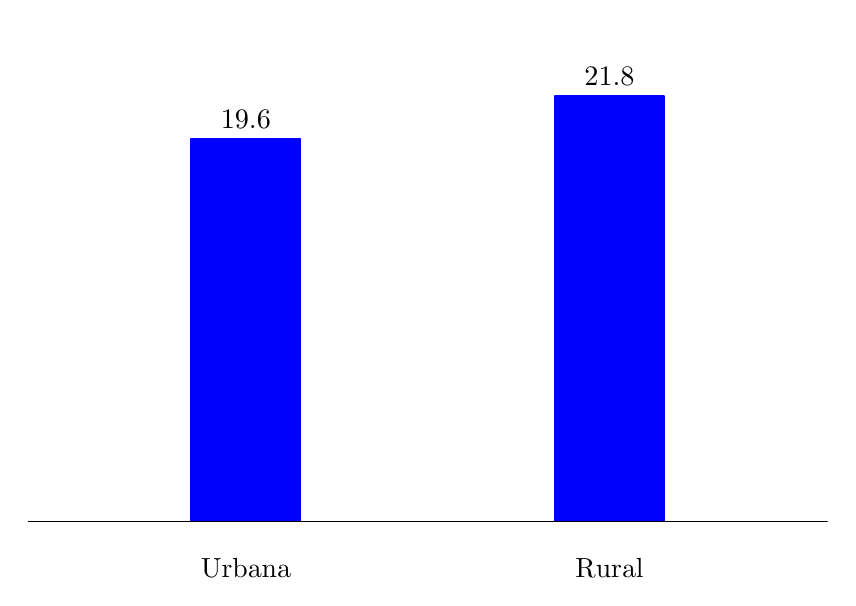
\begin{tikzpicture}[x=1pt,y=1pt]  % Created by tikzDevice version 0.9 on 2016-03-03 05:03:26
% !TEX encoding = UTF-8 Unicode
\definecolor{fillColor}{RGB}{255,255,255}
\path[use as bounding box,fill=fillColor,fill opacity=0.00] (0,0) rectangle (289.08,198.74);
\begin{scope}
\path[clip] (  0.00,  0.00) rectangle (289.08,198.74);

\path[] (  0.00,  0.00) rectangle (289.08,198.74);
\end{scope}
\begin{scope}
\path[clip] (  0.00,  0.00) rectangle (289.08,198.74);

\path[] (  0.00, 12.77) rectangle (289.08,181.67);

\path[] ( 78.84, 12.77) --
	( 78.84,181.67);

\path[] (210.24, 12.77) --
	(210.24,181.67);
\definecolor{drawColor}{RGB}{0,0,255}
\definecolor{fillColor}{RGB}{0,0,255}

\path[draw=drawColor,line width= 0.6pt,line join=round,fill=fillColor] ( 59.13, 20.44) rectangle ( 98.55,158.50);

\path[draw=drawColor,line width= 0.6pt,line join=round,fill=fillColor] (190.53, 20.44) rectangle (229.95,173.99);
\definecolor{drawColor}{RGB}{0,0,0}

\path[draw=drawColor,line width= 0.1pt,line join=round] (  0.00, 20.44) -- (289.08, 20.44);

\node[text=drawColor,anchor=base,inner sep=0pt, outer sep=0pt, scale=  1.02] at ( 78.84,162.47) {19.6};

\node[text=drawColor,anchor=base,inner sep=0pt, outer sep=0pt, scale=  1.02] at (210.24,177.96) {21.8};

\path[] (  0.00, 12.77) rectangle (289.08,181.67);
\end{scope}
\begin{scope}
\path[clip] (  0.00,  0.00) rectangle (289.08,198.74);

\path[] (  0.00, 12.77) --
	(289.08, 12.77);
\end{scope}
\begin{scope}
\path[clip] (  0.00,  0.00) rectangle (289.08,198.74);

\path[] ( 78.84, 10.02) --
	( 78.84, 12.77);

\path[] (210.24, 10.02) --
	(210.24, 12.77);
\end{scope}
\begin{scope}
\path[clip] (  0.00,  0.00) rectangle (289.08,198.74);
\definecolor{drawColor}{RGB}{0,0,0}

\node[text=drawColor,anchor=base,inner sep=0pt, outer sep=0pt, scale=  1.00] at ( 78.84, -0.00) {Urbana};

\node[text=drawColor,anchor=base,inner sep=0pt, outer sep=0pt, scale=  1.00] at (210.24, -0.00) {Rural};
\end{scope}
  \end{tikzpicture}
}%
{%
	ENSMI 2008/2009} %


%#########################3########################

\cajita{%
	Duración de la lactancia según etnia}%
{%
}%
{%
	Duración de cualquier tipo de lactancia en niños menores de 2 años según etnia de la madre} %
{%
	República de Guatemala, 2008/2009, en meses} %
{%
	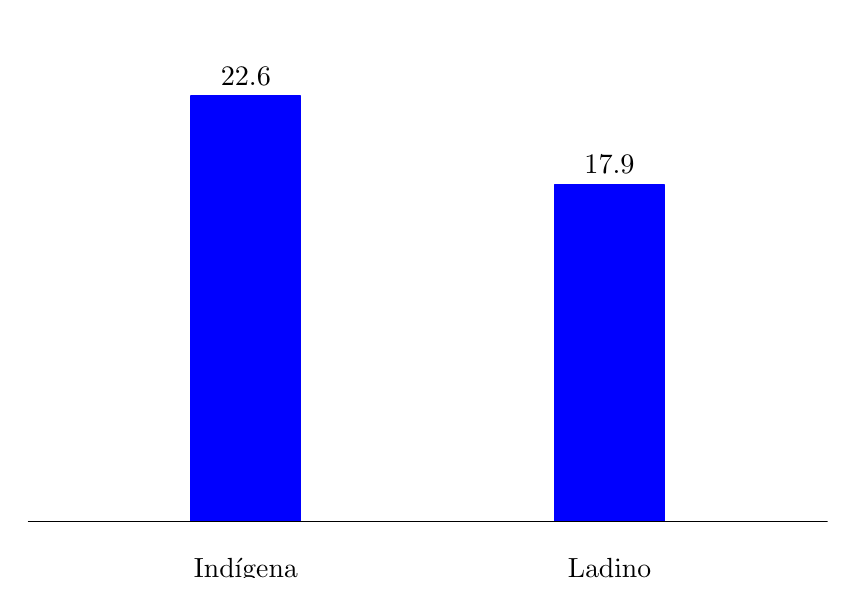
\begin{tikzpicture}[x=1pt,y=1pt]  % Created by tikzDevice version 0.9 on 2016-03-03 05:04:33
% !TEX encoding = UTF-8 Unicode
\definecolor{fillColor}{RGB}{255,255,255}
\path[use as bounding box,fill=fillColor,fill opacity=0.00] (0,0) rectangle (289.08,198.74);
\begin{scope}
\path[clip] (  0.00,  0.00) rectangle (289.08,198.74);

\path[] (  0.00,  0.00) rectangle (289.08,198.74);
\end{scope}
\begin{scope}
\path[clip] (  0.00,  0.00) rectangle (289.08,198.74);

\path[] (  0.00, 12.77) rectangle (289.08,181.67);

\path[] ( 78.84, 12.77) --
	( 78.84,181.67);

\path[] (210.24, 12.77) --
	(210.24,181.67);
\definecolor{drawColor}{RGB}{0,0,255}
\definecolor{fillColor}{RGB}{0,0,255}

\path[draw=drawColor,line width= 0.6pt,line join=round,fill=fillColor] ( 59.13, 20.44) rectangle ( 98.55,173.99);

\path[draw=drawColor,line width= 0.6pt,line join=round,fill=fillColor] (190.53, 20.44) rectangle (229.95,142.06);
\definecolor{drawColor}{RGB}{0,0,0}

\path[draw=drawColor,line width= 0.1pt,line join=round] (  0.00, 20.44) -- (289.08, 20.44);

\node[text=drawColor,anchor=base,inner sep=0pt, outer sep=0pt, scale=  1.02] at ( 78.84,177.96) {22.6};

\node[text=drawColor,anchor=base,inner sep=0pt, outer sep=0pt, scale=  1.02] at (210.24,146.03) {17.9};

\path[] (  0.00, 12.77) rectangle (289.08,181.67);
\end{scope}
\begin{scope}
\path[clip] (  0.00,  0.00) rectangle (289.08,198.74);

\path[] (  0.00, 12.77) --
	(289.08, 12.77);
\end{scope}
\begin{scope}
\path[clip] (  0.00,  0.00) rectangle (289.08,198.74);

\path[] ( 78.84, 10.02) --
	( 78.84, 12.77);

\path[] (210.24, 10.02) --
	(210.24, 12.77);
\end{scope}
\begin{scope}
\path[clip] (  0.00,  0.00) rectangle (289.08,198.74);
\definecolor{drawColor}{RGB}{0,0,0}

\node[text=drawColor,anchor=base,inner sep=0pt, outer sep=0pt, scale=  1.00] at ( 78.84, -0.00) {Indígena};

\node[text=drawColor,anchor=base,inner sep=0pt, outer sep=0pt, scale=  1.00] at (210.24, -0.00) {Ladino};
\end{scope}
  \end{tikzpicture}
}%
{%
	ENSMI 2008/2009} %

%#########################4########################

\cajita{%
	Duración de la lactancia por educación}%
{%
}%
{%
	Duración de cualquier tipo de lactancia en niños menores de 2 años según el grado de educación de la madre} %
{%
	República de Guatemala, 2008/2009, en meses} %
{%
	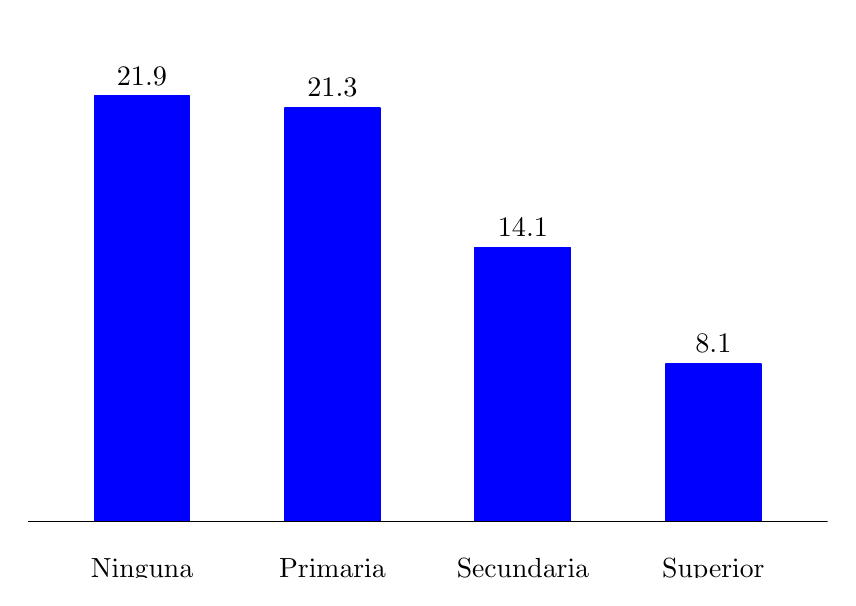
\begin{tikzpicture}[x=1pt,y=1pt]  % Created by tikzDevice version 0.9 on 2016-03-03 04:58:10
% !TEX encoding = UTF-8 Unicode
\definecolor{fillColor}{RGB}{255,255,255}
\path[use as bounding box,fill=fillColor,fill opacity=0.00] (0,0) rectangle (289.08,198.74);
\begin{scope}
\path[clip] (  0.00,  0.00) rectangle (289.08,198.74);

\path[] (  0.00,  0.00) rectangle (289.08,198.74);
\end{scope}
\begin{scope}
\path[clip] (  0.00,  0.00) rectangle (289.08,198.74);

\path[] (  0.00, 12.77) rectangle (289.08,181.67);

\path[] ( 41.30, 12.77) --
	( 41.30,181.67);

\path[] (110.13, 12.77) --
	(110.13,181.67);

\path[] (178.95, 12.77) --
	(178.95,181.67);

\path[] (247.78, 12.77) --
	(247.78,181.67);
\definecolor{drawColor}{RGB}{0,0,255}
\definecolor{fillColor}{RGB}{0,0,255}

\path[draw=drawColor,line width= 0.6pt,line join=round,fill=fillColor] ( 24.09, 20.44) rectangle ( 58.50,173.99);

\path[draw=drawColor,line width= 0.6pt,line join=round,fill=fillColor] ( 92.92, 20.44) rectangle (127.33,169.79);

\path[draw=drawColor,line width= 0.6pt,line join=round,fill=fillColor] (161.75, 20.44) rectangle (196.16,119.30);

\path[draw=drawColor,line width= 0.6pt,line join=round,fill=fillColor] (230.58, 20.44) rectangle (264.99, 77.24);
\definecolor{drawColor}{RGB}{0,0,0}

\path[draw=drawColor,line width= 0.1pt,line join=round] (  0.00, 20.44) -- (289.08, 20.44);

\node[text=drawColor,anchor=base,inner sep=0pt, outer sep=0pt, scale=  1.02] at ( 41.30,177.96) {21.9};

\node[text=drawColor,anchor=base,inner sep=0pt, outer sep=0pt, scale=  1.02] at (110.13,173.76) {21.3};

\node[text=drawColor,anchor=base,inner sep=0pt, outer sep=0pt, scale=  1.02] at (178.95,123.28) {14.1};

\node[text=drawColor,anchor=base,inner sep=0pt, outer sep=0pt, scale=  1.02] at (247.78, 81.21) {8.1};

\path[] (  0.00, 12.77) rectangle (289.08,181.67);
\end{scope}
\begin{scope}
\path[clip] (  0.00,  0.00) rectangle (289.08,198.74);

\path[] (  0.00, 12.77) --
	(289.08, 12.77);
\end{scope}
\begin{scope}
\path[clip] (  0.00,  0.00) rectangle (289.08,198.74);

\path[] ( 41.30, 10.02) --
	( 41.30, 12.77);

\path[] (110.13, 10.02) --
	(110.13, 12.77);

\path[] (178.95, 10.02) --
	(178.95, 12.77);

\path[] (247.78, 10.02) --
	(247.78, 12.77);
\end{scope}
\begin{scope}
\path[clip] (  0.00,  0.00) rectangle (289.08,198.74);
\definecolor{drawColor}{RGB}{0,0,0}

\node[text=drawColor,anchor=base,inner sep=0pt, outer sep=0pt, scale=  1.00] at ( 41.30, -0.00) {Ninguna};

\node[text=drawColor,anchor=base,inner sep=0pt, outer sep=0pt, scale=  1.00] at (110.13, -0.00) {Primaria};

\node[text=drawColor,anchor=base,inner sep=0pt, outer sep=0pt, scale=  1.00] at (178.95, -0.00) {Secundaria};

\node[text=drawColor,anchor=base,inner sep=0pt, outer sep=0pt, scale=  1.00] at (247.78, -0.00) {Superior};
\end{scope}
  \end{tikzpicture}
}%
{%
	ENSMI 2008/2009} %


%#########################5########################

\cajita{%
Niños de 0 a 3 meses según lactancia}%
{%
}%
{%
	Distribución de niños de 0 a 3 meses según lactancia y área de residencia
	} %
{%
	República de Guatemala, 2008/2009, en meses} %
{%
	\begin{tikzpicture}[x=1pt,y=1pt]  % Created by tikzDevice version 0.9 on 2016-03-03 04:58:13
% !TEX encoding = UTF-8 Unicode
\definecolor{fillColor}{RGB}{255,255,255}
\path[use as bounding box,fill=fillColor,fill opacity=0.00] (0,0) rectangle (289.08,198.74);
\begin{scope}
\path[clip] (  0.00,  0.00) rectangle (289.08,198.74);

\path[] (  0.00,  0.00) rectangle (289.08,198.74);
\end{scope}
\begin{scope}
\path[clip] (  0.00,  0.00) rectangle (289.08,198.74);

\path[] (  0.00, 18.46) rectangle (289.08,166.57);

\path[] ( 54.20, 18.46) --
	( 54.20,166.57);

\path[] (144.54, 18.46) --
	(144.54,166.57);

\path[] (234.88, 18.46) --
	(234.88,166.57);
\definecolor{drawColor}{RGB}{0,0,255}
\definecolor{fillColor}{RGB}{0,0,255}

\path[draw=drawColor,line width= 0.6pt,line join=round,fill=fillColor] ( 15.81, 18.46) rectangle ( 51.94, 30.54);
\definecolor{drawColor}{RGB}{157,187,255}
\definecolor{fillColor}{RGB}{157,187,255}

\path[draw=drawColor,line width= 0.6pt,line join=round,fill=fillColor] ( 56.46, 18.46) rectangle ( 92.60, 25.71);
\definecolor{drawColor}{RGB}{0,0,255}
\definecolor{fillColor}{RGB}{0,0,255}

\path[draw=drawColor,line width= 0.6pt,line join=round,fill=fillColor] (106.15, 18.46) rectangle (142.28,101.75);
\definecolor{drawColor}{RGB}{157,187,255}
\definecolor{fillColor}{RGB}{157,187,255}

\path[draw=drawColor,line width= 0.6pt,line join=round,fill=fillColor] (146.80, 18.46) rectangle (182.93,166.57);
\definecolor{drawColor}{RGB}{0,0,255}
\definecolor{fillColor}{RGB}{0,0,255}

\path[draw=drawColor,line width= 0.6pt,line join=round,fill=fillColor] (196.48, 18.46) rectangle (232.62, 72.08);
\definecolor{drawColor}{RGB}{157,187,255}
\definecolor{fillColor}{RGB}{157,187,255}

\path[draw=drawColor,line width= 0.6pt,line join=round,fill=fillColor] (237.14, 18.46) rectangle (273.27, 59.33);
\definecolor{drawColor}{RGB}{0,0,0}

\path[draw=drawColor,line width= 0.6pt,line join=round] (  0.00, 18.46) -- (289.08, 18.46);

\node[text=drawColor,rotate= 90.00,anchor=base west,inner sep=0pt, outer sep=0pt, scale=  0.83] at ( 37.11, 32.37) {5.5};

\node[text=drawColor,rotate= 90.00,anchor=base west,inner sep=0pt, outer sep=0pt, scale=  0.83] at ( 77.76, 27.53) {3.3};

\node[text=drawColor,rotate= 90.00,anchor=base west,inner sep=0pt, outer sep=0pt, scale=  0.83] at (127.45,104.29) {37.9};

\node[text=drawColor,rotate= 90.00,anchor=base west,inner sep=0pt, outer sep=0pt, scale=  0.83] at (168.10,169.12) {67.4};

\node[text=drawColor,rotate= 90.00,anchor=base west,inner sep=0pt, outer sep=0pt, scale=  0.83] at (217.79, 74.63) {24.4};

\node[text=drawColor,rotate= 90.00,anchor=base west,inner sep=0pt, outer sep=0pt, scale=  0.83] at (258.44, 61.88) {18.6};

\path[] (  0.00, 18.46) rectangle (289.08,166.57);
\end{scope}
\begin{scope}
\path[clip] (  0.00,  0.00) rectangle (289.08,198.74);

\path[] (  0.00, 18.46) --
	(289.08, 18.46);
\end{scope}
\begin{scope}
\path[clip] (  0.00,  0.00) rectangle (289.08,198.74);

\path[] ( 54.20, 15.71) --
	( 54.20, 18.46);

\path[] (144.54, 15.71) --
	(144.54, 18.46);

\path[] (234.88, 15.71) --
	(234.88, 18.46);
\end{scope}
\begin{scope}
\path[clip] (  0.00,  0.00) rectangle (289.08,198.74);
\definecolor{drawColor}{RGB}{0,0,0}

\node[text=drawColor,anchor=base,inner sep=0pt, outer sep=0pt, scale=  1.00] at ( 54.20,  5.69) {No lactando};

\node[text=drawColor,anchor=base,inner sep=0pt, outer sep=0pt, scale=  1.00] at (144.54,  5.69) {Lactancia Exclusiva};

\node[text=drawColor,anchor=base,inner sep=0pt, outer sep=0pt, scale=  1.00] at (234.88,  5.69) {Lactancia Predominante};
\end{scope}
\begin{scope}
\path[clip] (  0.00,  0.00) rectangle (289.08,198.74);
\coordinate (apoyo) at (57.27,191.13);
\coordinate (longitudFicticia) at (7.11,7.61);
\coordinate (longitud) at (7.11,7.11);
\coordinate (desX) at (142.24,0);
\coordinate (desY) at (0,0.25);
\definecolor[named]{ct1}{HTML}{
0000FF
}
\definecolor[named]{ct2}{HTML}{
9DBBFF
}
\definecolor[named]{ctb1}{HTML}{
0000FF
}
\definecolor[named]{ctb2}{HTML}{
9DBBFF
}
\path [fill=none] (apoyo) rectangle ($(apoyo)+(longitudFicticia)$)
node [xshift=0.3cm,inner sep=0pt, outer sep=0pt,midway,right,scale = 0.9]{Urbana};
\draw [color = ctb1,fill=ct1] ( $(apoyo)  + (desY) $) rectangle ($(apoyo)+ (desY) +(longitud)$);
\path [fill=none] ($(apoyo)+(desX)$) rectangle ($(apoyo)+(desX)+(longitudFicticia)$)
node [xshift=0.3cm,inner sep=0pt, outer sep=0pt,midway,right,scale = 0.9]{Rural};
\draw [color = ctb2 ,fill=ct2] ( $(apoyo)  + (desY) + (desX) $) rectangle ($(apoyo)+ (desY)+ (desX) +(longitud)$);
\end{scope}
  \end{tikzpicture}
}%
{%
	ENSMI 2008/2009} %


%#########################6########################

\cajita{%
	Niños de 0 a 3 meses según lactancia por etnia}%
{%
}%
{%
	Distribución de niños de 0 a 3 meses según lactancia y etnia
} %
{%
	República de Guatemala, 2008/2009, en meses} %
{%
	\begin{tikzpicture}[x=1pt,y=1pt]  % Created by tikzDevice version 0.9 on 2016-03-03 04:58:20
% !TEX encoding = UTF-8 Unicode
\definecolor{fillColor}{RGB}{255,255,255}
\path[use as bounding box,fill=fillColor,fill opacity=0.00] (0,0) rectangle (289.08,198.74);
\begin{scope}
\path[clip] (  0.00,  0.00) rectangle (289.08,198.74);

\path[] (  0.00,  0.00) rectangle (289.08,198.74);
\end{scope}
\begin{scope}
\path[clip] (  0.00,  0.00) rectangle (289.08,198.74);

\path[] (  0.00, 18.46) rectangle (289.08,164.23);

\path[] ( 54.20, 18.46) --
	( 54.20,164.23);

\path[] (144.54, 18.46) --
	(144.54,164.23);

\path[] (234.88, 18.46) --
	(234.88,164.23);
\definecolor{drawColor}{RGB}{0,0,255}
\definecolor{fillColor}{RGB}{0,0,255}

\path[draw=drawColor,line width= 0.6pt,line join=round,fill=fillColor] ( 15.81, 18.46) rectangle ( 51.94, 26.18);
\definecolor{drawColor}{RGB}{157,187,255}
\definecolor{fillColor}{RGB}{157,187,255}

\path[draw=drawColor,line width= 0.6pt,line join=round,fill=fillColor] ( 56.46, 18.46) rectangle ( 92.60, 27.61);
\definecolor{drawColor}{RGB}{0,0,255}
\definecolor{fillColor}{RGB}{0,0,255}

\path[draw=drawColor,line width= 0.6pt,line join=round,fill=fillColor] (106.15, 18.46) rectangle (142.28,164.23);
\definecolor{drawColor}{RGB}{157,187,255}
\definecolor{fillColor}{RGB}{157,187,255}

\path[draw=drawColor,line width= 0.6pt,line join=round,fill=fillColor] (146.80, 18.46) rectangle (182.93,102.43);
\definecolor{drawColor}{RGB}{0,0,255}
\definecolor{fillColor}{RGB}{0,0,255}

\path[draw=drawColor,line width= 0.6pt,line join=round,fill=fillColor] (196.48, 18.46) rectangle (232.62, 47.73);
\definecolor{drawColor}{RGB}{157,187,255}
\definecolor{fillColor}{RGB}{157,187,255}

\path[draw=drawColor,line width= 0.6pt,line join=round,fill=fillColor] (237.14, 18.46) rectangle (273.27, 72.74);
\definecolor{drawColor}{RGB}{0,0,0}

\path[draw=drawColor,line width= 0.6pt,line join=round] (  0.00, 18.46) -- (289.08, 18.46);

\node[text=drawColor,rotate= 90.00,anchor=base west,inner sep=0pt, outer sep=0pt, scale=  0.83] at ( 37.11, 28.01) {3.8};

\node[text=drawColor,rotate= 90.00,anchor=base west,inner sep=0pt, outer sep=0pt, scale=  0.83] at ( 77.76, 29.43) {4.5};

\node[text=drawColor,rotate= 90.00,anchor=base west,inner sep=0pt, outer sep=0pt, scale=  0.83] at (127.45,166.78) {71.7};

\node[text=drawColor,rotate= 90.00,anchor=base west,inner sep=0pt, outer sep=0pt, scale=  0.83] at (168.10,104.97) {41.3};

\node[text=drawColor,rotate= 90.00,anchor=base west,inner sep=0pt, outer sep=0pt, scale=  0.83] at (217.79, 50.28) {14.4};

\node[text=drawColor,rotate= 90.00,anchor=base west,inner sep=0pt, outer sep=0pt, scale=  0.83] at (258.44, 75.29) {26.7};

\path[] (  0.00, 18.46) rectangle (289.08,164.23);
\end{scope}
\begin{scope}
\path[clip] (  0.00,  0.00) rectangle (289.08,198.74);

\path[] (  0.00, 18.46) --
	(289.08, 18.46);
\end{scope}
\begin{scope}
\path[clip] (  0.00,  0.00) rectangle (289.08,198.74);

\path[] ( 54.20, 15.71) --
	( 54.20, 18.46);

\path[] (144.54, 15.71) --
	(144.54, 18.46);

\path[] (234.88, 15.71) --
	(234.88, 18.46);
\end{scope}
\begin{scope}
\path[clip] (  0.00,  0.00) rectangle (289.08,198.74);
\definecolor{drawColor}{RGB}{0,0,0}

\node[text=drawColor,anchor=base,inner sep=0pt, outer sep=0pt, scale=  1.00] at ( 54.20,  5.69) {No lactando};

\node[text=drawColor,anchor=base,inner sep=0pt, outer sep=0pt, scale=  1.00] at (144.54,  5.69) {Lactancia Exclusiva};

\node[text=drawColor,anchor=base,inner sep=0pt, outer sep=0pt, scale=  1.00] at (234.88,  5.69) {Lactancia Predominante};
\end{scope}
\begin{scope}
\path[clip] (  0.00,  0.00) rectangle (289.08,198.74);
\coordinate (apoyo) at (55.19,188.79);
\coordinate (longitudFicticia) at (7.11,9.95);
\coordinate (longitud) at (7.11,7.11);
\coordinate (desX) at (133.24,0);
\coordinate (desY) at (0,1.42);
\definecolor[named]{ct1}{HTML}{
0000FF
}
\definecolor[named]{ct2}{HTML}{
9DBBFF
}
\definecolor[named]{ctb1}{HTML}{
0000FF
}
\definecolor[named]{ctb2}{HTML}{
9DBBFF
}
\path [fill=none] (apoyo) rectangle ($(apoyo)+(longitudFicticia)$)
node [xshift=0.3cm,inner sep=0pt, outer sep=0pt,midway,right,scale = 0.9]{Indígena};
\draw [color = ctb1,fill=ct1] ( $(apoyo)  + (desY) $) rectangle ($(apoyo)+ (desY) +(longitud)$);
\path [fill=none] ($(apoyo)+(desX)$) rectangle ($(apoyo)+(desX)+(longitudFicticia)$)
node [xshift=0.3cm,inner sep=0pt, outer sep=0pt,midway,right,scale = 0.9]{No indígena};
\draw [color = ctb2 ,fill=ct2] ( $(apoyo)  + (desY) + (desX) $) rectangle ($(apoyo)+ (desY)+ (desX) +(longitud)$);
\end{scope}
  \end{tikzpicture}
}%
{%
	ENSMI 2008/2009} %


%#########################7########################

\cajita{%
	Niños de 0 a 3 meses según lactancia y educación de la madre}%
{%
}%
{%
	Distribución de niños de 0 a 3 meses según lactancia y educación de la madre
} %
{%
	República de Guatemala, 2008/2009, en meses} %
{%
	\begin{tikzpicture}[x=1pt,y=1pt]  % Created by tikzDevice version 0.9 on 2016-03-03 04:58:26
% !TEX encoding = UTF-8 Unicode
\definecolor{fillColor}{RGB}{255,255,255}
\path[use as bounding box,fill=fillColor,fill opacity=0.00] (0,0) rectangle (289.08,198.74);
\begin{scope}
\path[clip] (  0.00,  0.00) rectangle (289.08,198.74);

\path[] (  0.00,  0.00) rectangle (289.08,198.74);
\end{scope}
\begin{scope}
\path[clip] (  0.00,  0.00) rectangle (289.08,198.74);

\path[] (  0.00, 18.46) rectangle (289.08,164.65);

\path[] ( 54.20, 18.46) --
	( 54.20,164.65);

\path[] (144.54, 18.46) --
	(144.54,164.65);

\path[] (234.88, 18.46) --
	(234.88,164.65);
\definecolor{drawColor}{RGB}{0,0,255}
\definecolor{fillColor}{RGB}{0,0,255}

\path[draw=drawColor,line width= 0.6pt,line join=round,fill=fillColor] ( 15.81, 18.46) rectangle ( 51.94, 26.28);
\definecolor{drawColor}{RGB}{157,187,255}
\definecolor{fillColor}{RGB}{157,187,255}

\path[draw=drawColor,line width= 0.6pt,line join=round,fill=fillColor] ( 56.46, 18.46) rectangle ( 92.60, 26.93);
\definecolor{drawColor}{RGB}{0,0,255}
\definecolor{fillColor}{RGB}{0,0,255}

\path[draw=drawColor,line width= 0.6pt,line join=round,fill=fillColor] (106.15, 18.46) rectangle (142.28,164.65);
\definecolor{drawColor}{RGB}{157,187,255}
\definecolor{fillColor}{RGB}{157,187,255}

\path[draw=drawColor,line width= 0.6pt,line join=round,fill=fillColor] (146.80, 18.46) rectangle (182.93, 30.84);
\definecolor{drawColor}{RGB}{0,0,255}
\definecolor{fillColor}{RGB}{0,0,255}

\path[draw=drawColor,line width= 0.6pt,line join=round,fill=fillColor] (196.48, 18.46) rectangle (232.62, 67.33);
\definecolor{drawColor}{RGB}{157,187,255}
\definecolor{fillColor}{RGB}{157,187,255}

\path[draw=drawColor,line width= 0.6pt,line join=round,fill=fillColor] (237.14, 18.46) rectangle (273.27, 44.52);
\definecolor{drawColor}{RGB}{0,0,0}

\path[draw=drawColor,line width= 0.6pt,line join=round] (  0.00, 18.46) -- (289.08, 18.46);

\node[text=drawColor,rotate= 90.00,anchor=base west,inner sep=0pt, outer sep=0pt, scale=  0.83] at ( 37.11, 28.10) {3.6};

\node[text=drawColor,rotate= 90.00,anchor=base west,inner sep=0pt, outer sep=0pt, scale=  0.83] at ( 77.76, 28.75) {3.9};

\node[text=drawColor,rotate= 90.00,anchor=base west,inner sep=0pt, outer sep=0pt, scale=  0.83] at (127.45,167.20) {67.3};

\node[text=drawColor,rotate= 90.00,anchor=base west,inner sep=0pt, outer sep=0pt, scale=  0.83] at (168.10, 32.66) {5.7};

\node[text=drawColor,rotate= 90.00,anchor=base west,inner sep=0pt, outer sep=0pt, scale=  0.83] at (217.79, 69.88) {22.5};

\node[text=drawColor,rotate= 90.00,anchor=base west,inner sep=0pt, outer sep=0pt, scale=  0.83] at (258.44, 47.07) {12.0};

\path[] (  0.00, 18.46) rectangle (289.08,164.65);
\end{scope}
\begin{scope}
\path[clip] (  0.00,  0.00) rectangle (289.08,198.74);

\path[] (  0.00, 18.46) --
	(289.08, 18.46);
\end{scope}
\begin{scope}
\path[clip] (  0.00,  0.00) rectangle (289.08,198.74);

\path[] ( 54.20, 15.71) --
	( 54.20, 18.46);

\path[] (144.54, 15.71) --
	(144.54, 18.46);

\path[] (234.88, 15.71) --
	(234.88, 18.46);
\end{scope}
\begin{scope}
\path[clip] (  0.00,  0.00) rectangle (289.08,198.74);
\definecolor{drawColor}{RGB}{0,0,0}

\node[text=drawColor,anchor=base,inner sep=0pt, outer sep=0pt, scale=  1.00] at ( 54.20,  5.69) {No lactando};

\node[text=drawColor,anchor=base,inner sep=0pt, outer sep=0pt, scale=  1.00] at (144.54,  5.69) {Lactancia Exclusiva};

\node[text=drawColor,anchor=base,inner sep=0pt, outer sep=0pt, scale=  1.00] at (234.88,  5.69) {Lactancia Predominante};
\end{scope}
\begin{scope}
\path[clip] (  0.00,  0.00) rectangle (289.08,198.74);
\coordinate (apoyo) at (46.95,189.2);
\coordinate (longitudFicticia) at (7.11,9.54);
\coordinate (longitud) at (7.11,7.11);
\coordinate (desX) at (147.1,0);
\coordinate (desY) at (0,1.21);
\definecolor[named]{ct1}{HTML}{
0000FF
}
\definecolor[named]{ct2}{HTML}{
9DBBFF
}
\definecolor[named]{ctb1}{HTML}{
0000FF
}
\definecolor[named]{ctb2}{HTML}{
9DBBFF
}
\path [fill=none] (apoyo) rectangle ($(apoyo)+(longitudFicticia)$)
node [xshift=0.3cm,inner sep=0pt, outer sep=0pt,midway,right,scale = 0.9]{Sin educación};
\draw [color = ctb1,fill=ct1] ( $(apoyo)  + (desY) $) rectangle ($(apoyo)+ (desY) +(longitud)$);
\path [fill=none] ($(apoyo)+(desX)$) rectangle ($(apoyo)+(desX)+(longitudFicticia)$)
node [xshift=0.3cm,inner sep=0pt, outer sep=0pt,midway,right,scale = 0.9]{Superior};
\draw [color = ctb2 ,fill=ct2] ( $(apoyo)  + (desY) + (desX) $) rectangle ($(apoyo)+ (desY)+ (desX) +(longitud)$);
\end{scope}
  \end{tikzpicture}
}%
{%
	ENSMI 2008/2009} %

%#########################8########################

\cajita{%
	Niños de 0 a 5 meses según lactancia}%
{%
}%
{%
	Distribución de niños de 0 a 5 meses según lactancia y área de residencia
} %
{%
	República de Guatemala, 2008/2009, en meses} %
{%
	\begin{tikzpicture}[x=1pt,y=1pt]  % Created by tikzDevice version 0.9 on 2016-03-03 04:58:32
% !TEX encoding = UTF-8 Unicode
\definecolor{fillColor}{RGB}{255,255,255}
\path[use as bounding box,fill=fillColor,fill opacity=0.00] (0,0) rectangle (289.08,198.74);
\begin{scope}
\path[clip] (  0.00,  0.00) rectangle (289.08,198.74);

\path[] (  0.00,  0.00) rectangle (289.08,198.74);
\end{scope}
\begin{scope}
\path[clip] (  0.00,  0.00) rectangle (289.08,198.74);

\path[] (  0.00, 18.46) rectangle (289.08,166.57);

\path[] ( 54.20, 18.46) --
	( 54.20,166.57);

\path[] (144.54, 18.46) --
	(144.54,166.57);

\path[] (234.88, 18.46) --
	(234.88,166.57);
\definecolor{drawColor}{RGB}{0,0,255}
\definecolor{fillColor}{RGB}{0,0,255}

\path[draw=drawColor,line width= 0.6pt,line join=round,fill=fillColor] ( 15.81, 18.46) rectangle ( 51.94, 42.73);
\definecolor{drawColor}{RGB}{157,187,255}
\definecolor{fillColor}{RGB}{157,187,255}

\path[draw=drawColor,line width= 0.6pt,line join=round,fill=fillColor] ( 56.46, 18.46) rectangle ( 92.60, 26.80);
\definecolor{drawColor}{RGB}{0,0,255}
\definecolor{fillColor}{RGB}{0,0,255}

\path[draw=drawColor,line width= 0.6pt,line join=round,fill=fillColor] (106.15, 18.46) rectangle (142.28, 98.16);
\definecolor{drawColor}{RGB}{157,187,255}
\definecolor{fillColor}{RGB}{157,187,255}

\path[draw=drawColor,line width= 0.6pt,line join=round,fill=fillColor] (146.80, 18.46) rectangle (182.93,166.57);
\definecolor{drawColor}{RGB}{0,0,255}
\definecolor{fillColor}{RGB}{0,0,255}

\path[draw=drawColor,line width= 0.6pt,line join=round,fill=fillColor] (196.48, 18.46) rectangle (232.62, 73.88);
\definecolor{drawColor}{RGB}{157,187,255}
\definecolor{fillColor}{RGB}{157,187,255}

\path[draw=drawColor,line width= 0.6pt,line join=round,fill=fillColor] (237.14, 18.46) rectangle (273.27, 61.13);
\definecolor{drawColor}{RGB}{0,0,0}

\path[draw=drawColor,line width= 0.6pt,line join=round] (  0.00, 18.46) -- (289.08, 18.46);

\node[text=drawColor,rotate= 90.00,anchor=base west,inner sep=0pt, outer sep=0pt, scale=  0.83] at ( 37.11, 44.56) {9.9};

\node[text=drawColor,rotate= 90.00,anchor=base west,inner sep=0pt, outer sep=0pt, scale=  0.83] at ( 77.76, 28.62) {3.4};

\node[text=drawColor,rotate= 90.00,anchor=base west,inner sep=0pt, outer sep=0pt, scale=  0.83] at (127.45,100.70) {32.5};

\node[text=drawColor,rotate= 90.00,anchor=base west,inner sep=0pt, outer sep=0pt, scale=  0.83] at (168.10,169.12) {60.4};

\node[text=drawColor,rotate= 90.00,anchor=base west,inner sep=0pt, outer sep=0pt, scale=  0.83] at (217.79, 76.43) {22.6};

\node[text=drawColor,rotate= 90.00,anchor=base west,inner sep=0pt, outer sep=0pt, scale=  0.83] at (258.44, 63.68) {17.4};

\path[] (  0.00, 18.46) rectangle (289.08,166.57);
\end{scope}
\begin{scope}
\path[clip] (  0.00,  0.00) rectangle (289.08,198.74);

\path[] (  0.00, 18.46) --
	(289.08, 18.46);
\end{scope}
\begin{scope}
\path[clip] (  0.00,  0.00) rectangle (289.08,198.74);

\path[] ( 54.20, 15.71) --
	( 54.20, 18.46);

\path[] (144.54, 15.71) --
	(144.54, 18.46);

\path[] (234.88, 15.71) --
	(234.88, 18.46);
\end{scope}
\begin{scope}
\path[clip] (  0.00,  0.00) rectangle (289.08,198.74);
\definecolor{drawColor}{RGB}{0,0,0}

\node[text=drawColor,anchor=base,inner sep=0pt, outer sep=0pt, scale=  1.00] at ( 54.20,  5.69) {No lactando};

\node[text=drawColor,anchor=base,inner sep=0pt, outer sep=0pt, scale=  1.00] at (144.54,  5.69) {Lactancia Exclusiva};

\node[text=drawColor,anchor=base,inner sep=0pt, outer sep=0pt, scale=  1.00] at (234.88,  5.69) {Lactancia Predominante};
\end{scope}
\begin{scope}
\path[clip] (  0.00,  0.00) rectangle (289.08,198.74);
\coordinate (apoyo) at (57.27,191.13);
\coordinate (longitudFicticia) at (7.11,7.61);
\coordinate (longitud) at (7.11,7.11);
\coordinate (desX) at (142.24,0);
\coordinate (desY) at (0,0.25);
\definecolor[named]{ct1}{HTML}{
0000FF
}
\definecolor[named]{ct2}{HTML}{
9DBBFF
}
\definecolor[named]{ctb1}{HTML}{
0000FF
}
\definecolor[named]{ctb2}{HTML}{
9DBBFF
}
\path [fill=none] (apoyo) rectangle ($(apoyo)+(longitudFicticia)$)
node [xshift=0.3cm,inner sep=0pt, outer sep=0pt,midway,right,scale = 0.9]{Urbana};
\draw [color = ctb1,fill=ct1] ( $(apoyo)  + (desY) $) rectangle ($(apoyo)+ (desY) +(longitud)$);
\path [fill=none] ($(apoyo)+(desX)$) rectangle ($(apoyo)+(desX)+(longitudFicticia)$)
node [xshift=0.3cm,inner sep=0pt, outer sep=0pt,midway,right,scale = 0.9]{Rural};
\draw [color = ctb2 ,fill=ct2] ( $(apoyo)  + (desY) + (desX) $) rectangle ($(apoyo)+ (desY)+ (desX) +(longitud)$);
\end{scope}
  \end{tikzpicture}
}%
{%
	ENSMI 2008/2009} %


%#########################9########################

\cajita{%
	Niños de 0 a 5 meses según lactancia por etnia}%
{%
}%
{%
	Distribución de niños de 0 a 5 meses según lactancia y etnia
} %
{%
	República de Guatemala, 2008/2009, en meses} %
{%
	\begin{tikzpicture}[x=1pt,y=1pt]  % Created by tikzDevice version 0.9 on 2016-03-03 04:58:38
% !TEX encoding = UTF-8 Unicode
\definecolor{fillColor}{RGB}{255,255,255}
\path[use as bounding box,fill=fillColor,fill opacity=0.00] (0,0) rectangle (289.08,198.74);
\begin{scope}
\path[clip] (  0.00,  0.00) rectangle (289.08,198.74);

\path[] (  0.00,  0.00) rectangle (289.08,198.74);
\end{scope}
\begin{scope}
\path[clip] (  0.00,  0.00) rectangle (289.08,198.74);

\path[] (  0.00, 18.46) rectangle (289.08,164.23);

\path[] ( 54.20, 18.46) --
	( 54.20,164.23);

\path[] (144.54, 18.46) --
	(144.54,164.23);

\path[] (234.88, 18.46) --
	(234.88,164.23);
\definecolor{drawColor}{RGB}{0,0,255}
\definecolor{fillColor}{RGB}{0,0,255}

\path[draw=drawColor,line width= 0.6pt,line join=round,fill=fillColor] ( 15.81, 18.46) rectangle ( 51.94, 25.48);
\definecolor{drawColor}{RGB}{157,187,255}
\definecolor{fillColor}{RGB}{157,187,255}

\path[draw=drawColor,line width= 0.6pt,line join=round,fill=fillColor] ( 56.46, 18.46) rectangle ( 92.60, 36.90);
\definecolor{drawColor}{RGB}{0,0,255}
\definecolor{fillColor}{RGB}{0,0,255}

\path[draw=drawColor,line width= 0.6pt,line join=round,fill=fillColor] (106.15, 18.46) rectangle (142.28,164.23);
\definecolor{drawColor}{RGB}{157,187,255}
\definecolor{fillColor}{RGB}{157,187,255}

\path[draw=drawColor,line width= 0.6pt,line join=round,fill=fillColor] (146.80, 18.46) rectangle (182.93, 93.98);
\definecolor{drawColor}{RGB}{0,0,255}
\definecolor{fillColor}{RGB}{0,0,255}

\path[draw=drawColor,line width= 0.6pt,line join=round,fill=fillColor] (196.48, 18.46) rectangle (232.62, 52.49);
\definecolor{drawColor}{RGB}{157,187,255}
\definecolor{fillColor}{RGB}{157,187,255}

\path[draw=drawColor,line width= 0.6pt,line join=round,fill=fillColor] (237.14, 18.46) rectangle (273.27, 68.95);
\definecolor{drawColor}{RGB}{0,0,0}

\path[draw=drawColor,line width= 0.6pt,line join=round] (  0.00, 18.46) -- (289.08, 18.46);

\node[text=drawColor,rotate= 90.00,anchor=base west,inner sep=0pt, outer sep=0pt, scale=  0.83] at ( 37.11, 27.31) {3.2};

\node[text=drawColor,rotate= 90.00,anchor=base west,inner sep=0pt, outer sep=0pt, scale=  0.83] at ( 77.76, 38.72) {8.4};

\node[text=drawColor,rotate= 90.00,anchor=base west,inner sep=0pt, outer sep=0pt, scale=  0.83] at (127.45,166.78) {66.4};

\node[text=drawColor,rotate= 90.00,anchor=base west,inner sep=0pt, outer sep=0pt, scale=  0.83] at (168.10, 96.53) {34.4};

\node[text=drawColor,rotate= 90.00,anchor=base west,inner sep=0pt, outer sep=0pt, scale=  0.83] at (217.79, 55.03) {15.5};

\node[text=drawColor,rotate= 90.00,anchor=base west,inner sep=0pt, outer sep=0pt, scale=  0.83] at (258.44, 71.50) {23.0};

\path[] (  0.00, 18.46) rectangle (289.08,164.23);
\end{scope}
\begin{scope}
\path[clip] (  0.00,  0.00) rectangle (289.08,198.74);

\path[] (  0.00, 18.46) --
	(289.08, 18.46);
\end{scope}
\begin{scope}
\path[clip] (  0.00,  0.00) rectangle (289.08,198.74);

\path[] ( 54.20, 15.71) --
	( 54.20, 18.46);

\path[] (144.54, 15.71) --
	(144.54, 18.46);

\path[] (234.88, 15.71) --
	(234.88, 18.46);
\end{scope}
\begin{scope}
\path[clip] (  0.00,  0.00) rectangle (289.08,198.74);
\definecolor{drawColor}{RGB}{0,0,0}

\node[text=drawColor,anchor=base,inner sep=0pt, outer sep=0pt, scale=  1.00] at ( 54.20,  5.69) {No lactando};

\node[text=drawColor,anchor=base,inner sep=0pt, outer sep=0pt, scale=  1.00] at (144.54,  5.69) {Lactancia Exclusiva};

\node[text=drawColor,anchor=base,inner sep=0pt, outer sep=0pt, scale=  1.00] at (234.88,  5.69) {Lactancia Predominante};
\end{scope}
\begin{scope}
\path[clip] (  0.00,  0.00) rectangle (289.08,198.74);
\coordinate (apoyo) at (55.19,188.79);
\coordinate (longitudFicticia) at (7.11,9.95);
\coordinate (longitud) at (7.11,7.11);
\coordinate (desX) at (133.24,0);
\coordinate (desY) at (0,1.42);
\definecolor[named]{ct1}{HTML}{
0000FF
}
\definecolor[named]{ct2}{HTML}{
9DBBFF
}
\definecolor[named]{ctb1}{HTML}{
0000FF
}
\definecolor[named]{ctb2}{HTML}{
9DBBFF
}
\path [fill=none] (apoyo) rectangle ($(apoyo)+(longitudFicticia)$)
node [xshift=0.3cm,inner sep=0pt, outer sep=0pt,midway,right,scale = 0.9]{Indígena};
\draw [color = ctb1,fill=ct1] ( $(apoyo)  + (desY) $) rectangle ($(apoyo)+ (desY) +(longitud)$);
\path [fill=none] ($(apoyo)+(desX)$) rectangle ($(apoyo)+(desX)+(longitudFicticia)$)
node [xshift=0.3cm,inner sep=0pt, outer sep=0pt,midway,right,scale = 0.9]{No indígena};
\draw [color = ctb2 ,fill=ct2] ( $(apoyo)  + (desY) + (desX) $) rectangle ($(apoyo)+ (desY)+ (desX) +(longitud)$);
\end{scope}
  \end{tikzpicture}
}%
{%
	ENSMI 2008/2009} %


%#########################10########################

\cajita{%
	Niños de 0 a 5 meses según lactancia y educación de la madre}%
{%
}%
{%
	Distribución de niños de 0 a 5 meses según lactancia y educación de la madre
} %
{%
	República de Guatemala, 2008/2009, en meses} %
{%
	\begin{tikzpicture}[x=1pt,y=1pt]  % Created by tikzDevice version 0.9 on 2016-03-03 04:58:43
% !TEX encoding = UTF-8 Unicode
\definecolor{fillColor}{RGB}{255,255,255}
\path[use as bounding box,fill=fillColor,fill opacity=0.00] (0,0) rectangle (289.08,198.74);
\begin{scope}
\path[clip] (  0.00,  0.00) rectangle (289.08,198.74);

\path[] (  0.00,  0.00) rectangle (289.08,198.74);
\end{scope}
\begin{scope}
\path[clip] (  0.00,  0.00) rectangle (289.08,198.74);

\path[] (  0.00, 18.46) rectangle (289.08,164.65);

\path[] ( 54.20, 18.46) --
	( 54.20,164.65);

\path[] (144.54, 18.46) --
	(144.54,164.65);

\path[] (234.88, 18.46) --
	(234.88,164.65);
\definecolor{drawColor}{RGB}{0,0,255}
\definecolor{fillColor}{RGB}{0,0,255}

\path[draw=drawColor,line width= 0.6pt,line join=round,fill=fillColor] ( 15.81, 18.46) rectangle ( 51.94, 25.31);
\definecolor{drawColor}{RGB}{157,187,255}
\definecolor{fillColor}{RGB}{157,187,255}

\path[draw=drawColor,line width= 0.6pt,line join=round,fill=fillColor] ( 56.46, 18.46) rectangle ( 92.60, 38.79);
\definecolor{drawColor}{RGB}{0,0,255}
\definecolor{fillColor}{RGB}{0,0,255}

\path[draw=drawColor,line width= 0.6pt,line join=round,fill=fillColor] (106.15, 18.46) rectangle (142.28,164.65);
\definecolor{drawColor}{RGB}{157,187,255}
\definecolor{fillColor}{RGB}{157,187,255}

\path[draw=drawColor,line width= 0.6pt,line join=round,fill=fillColor] (146.80, 18.46) rectangle (182.93, 29.19);
\definecolor{drawColor}{RGB}{0,0,255}
\definecolor{fillColor}{RGB}{0,0,255}

\path[draw=drawColor,line width= 0.6pt,line join=round,fill=fillColor] (196.48, 18.46) rectangle (232.62, 63.91);
\definecolor{drawColor}{RGB}{157,187,255}
\definecolor{fillColor}{RGB}{157,187,255}

\path[draw=drawColor,line width= 0.6pt,line join=round,fill=fillColor] (237.14, 18.46) rectangle (273.27, 41.07);
\definecolor{drawColor}{RGB}{0,0,0}

\path[draw=drawColor,line width= 0.6pt,line join=round] (  0.00, 18.46) -- (289.08, 18.46);

\node[text=drawColor,rotate= 90.00,anchor=base west,inner sep=0pt, outer sep=0pt, scale=  0.83] at ( 37.11, 27.13) {3.0};

\node[text=drawColor,rotate= 90.00,anchor=base west,inner sep=0pt, outer sep=0pt, scale=  0.83] at ( 77.76, 40.61) {8.9};

\node[text=drawColor,rotate= 90.00,anchor=base west,inner sep=0pt, outer sep=0pt, scale=  0.83] at (127.45,167.20) {64.0};

\node[text=drawColor,rotate= 90.00,anchor=base west,inner sep=0pt, outer sep=0pt, scale=  0.83] at (168.10, 31.02) {4.7};

\node[text=drawColor,rotate= 90.00,anchor=base west,inner sep=0pt, outer sep=0pt, scale=  0.83] at (217.79, 66.46) {19.9};

\node[text=drawColor,rotate= 90.00,anchor=base west,inner sep=0pt, outer sep=0pt, scale=  0.83] at (258.44, 42.89) {9.9};

\path[] (  0.00, 18.46) rectangle (289.08,164.65);
\end{scope}
\begin{scope}
\path[clip] (  0.00,  0.00) rectangle (289.08,198.74);

\path[] (  0.00, 18.46) --
	(289.08, 18.46);
\end{scope}
\begin{scope}
\path[clip] (  0.00,  0.00) rectangle (289.08,198.74);

\path[] ( 54.20, 15.71) --
	( 54.20, 18.46);

\path[] (144.54, 15.71) --
	(144.54, 18.46);

\path[] (234.88, 15.71) --
	(234.88, 18.46);
\end{scope}
\begin{scope}
\path[clip] (  0.00,  0.00) rectangle (289.08,198.74);
\definecolor{drawColor}{RGB}{0,0,0}

\node[text=drawColor,anchor=base,inner sep=0pt, outer sep=0pt, scale=  1.00] at ( 54.20,  5.69) {No lactando};

\node[text=drawColor,anchor=base,inner sep=0pt, outer sep=0pt, scale=  1.00] at (144.54,  5.69) {Lactancia Exclusiva};

\node[text=drawColor,anchor=base,inner sep=0pt, outer sep=0pt, scale=  1.00] at (234.88,  5.69) {Lactancia Predominante};
\end{scope}
\begin{scope}
\path[clip] (  0.00,  0.00) rectangle (289.08,198.74);
\coordinate (apoyo) at (46.95,189.2);
\coordinate (longitudFicticia) at (7.11,9.54);
\coordinate (longitud) at (7.11,7.11);
\coordinate (desX) at (147.1,0);
\coordinate (desY) at (0,1.21);
\definecolor[named]{ct1}{HTML}{
0000FF
}
\definecolor[named]{ct2}{HTML}{
9DBBFF
}
\definecolor[named]{ctb1}{HTML}{
0000FF
}
\definecolor[named]{ctb2}{HTML}{
9DBBFF
}
\path [fill=none] (apoyo) rectangle ($(apoyo)+(longitudFicticia)$)
node [xshift=0.3cm,inner sep=0pt, outer sep=0pt,midway,right,scale = 0.9]{Sin educación};
\draw [color = ctb1,fill=ct1] ( $(apoyo)  + (desY) $) rectangle ($(apoyo)+ (desY) +(longitud)$);
\path [fill=none] ($(apoyo)+(desX)$) rectangle ($(apoyo)+(desX)+(longitudFicticia)$)
node [xshift=0.3cm,inner sep=0pt, outer sep=0pt,midway,right,scale = 0.9]{Superior};
\draw [color = ctb2 ,fill=ct2] ( $(apoyo)  + (desY) + (desX) $) rectangle ($(apoyo)+ (desY)+ (desX) +(longitud)$);
\end{scope}
  \end{tikzpicture}
}%
{%
	ENSMI 2008/2009} %